\section{Анализ требований к программному средству и разработка функциональных требований}
\label{sec:domain}

\subsection{Функциональная модель программного средства}
\label{sec:domain:model}

Функциональная модель программного средства представлена в виде схемы алгоритма игрового процесса и диаграммы вариантов использования. Алгоритм игрового 
процесса показывает как будет идти игровой процесс в зависимости от действий игроков. Варианты использования отражают функциональность системы в ответ на внешние 
воздействия с точки зрения получения значимого результата для пользователей.

\subsubsection{} Анализ игрового процесса
\label{sec:domain:model:game}

Перед началом проектирования необходимо проанализировать игровой процесс и определить его цикл. Целесообразным будет проведение анализа как с точки зрения игрока, так и 
с точки зрения организатора. Результат анализа представлен в виде схем алгоритмов на рисунках \ref{fig:domain:model:game:player_alg} для игрока 
и \ref{fig:domain:model:game:organizer_alg} для организатора. 
Схема ограничивается лишь непосредственно игровым циклом и не включает в себя процесс авторизации и установки соединения с игровым лобби.

\begin{figure}
\centering
	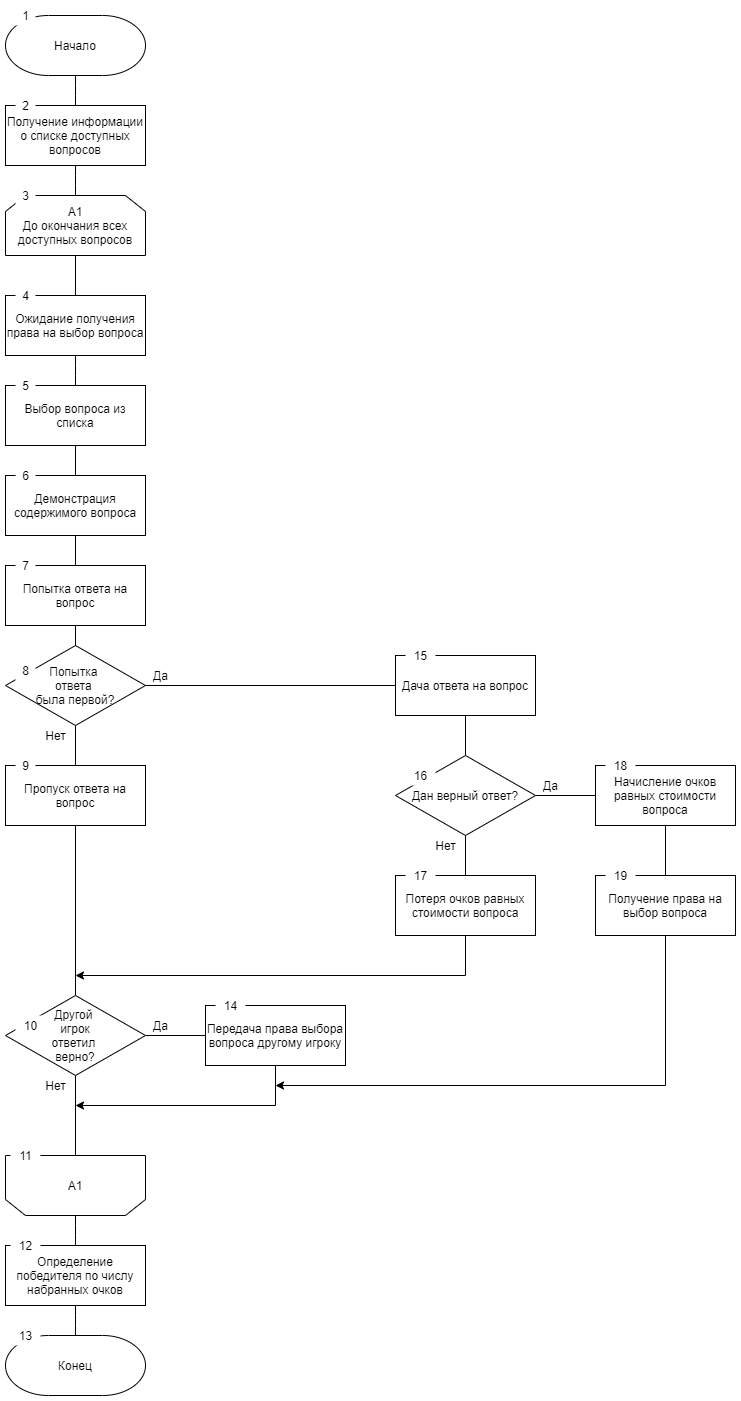
\includegraphics[scale=0.7]{attachments/game_player_alg.png}
	\caption{Схема алгоритма игрового процесса с точки зрения игрока}
	\label{fig:domain:model:game:player_alg}
\end{figure}

\begin{figure}
\centering
	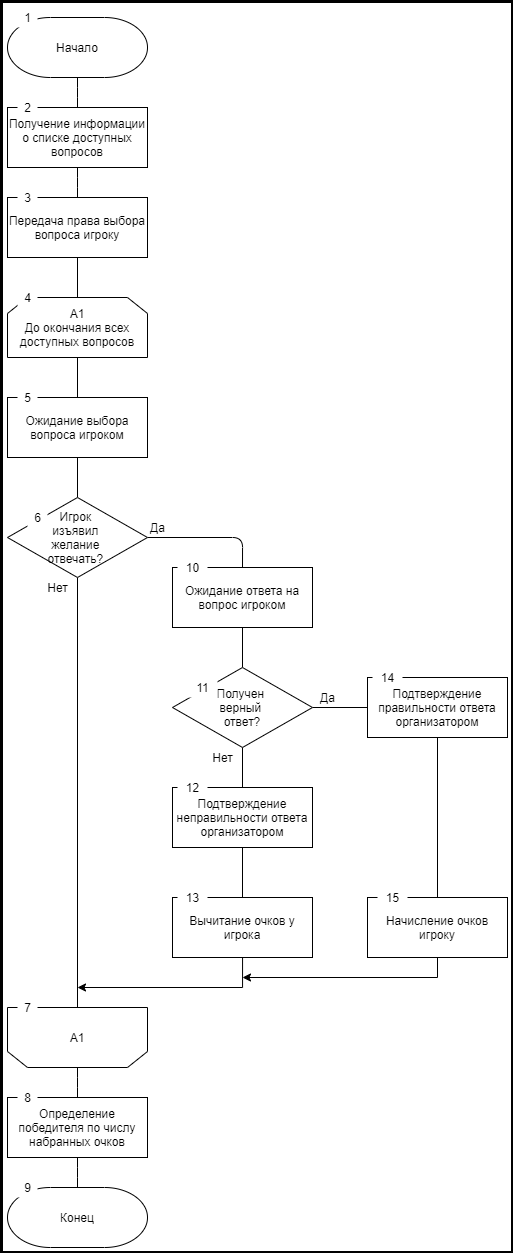
\includegraphics[scale=0.7]{attachments/game_organizer_alg.png}
	\caption{Схема алгоритма игрового процесса с точки зрения организатора}
	\label{fig:domain:model:game:organizer_alg}
\end{figure}

Одной из особенностей данных схем является цикличность, с которой проходит игровой процесс. 

Цикл для игрока начинается с того, что игрок получает право на выбор вопроса из списка, после сделанного выбора все игроки видят содержимое вопроса и тот, кто первый 
сможет дать правильный ответ на вопрос и получит сумму баллов на свой игровой счет. В случае неправильного ответа на вопрос баллы вычитаются из игрового счета.
Здесь стоит обратить внимание на то, что игрок, выбравший вопрос не получает никакого игрового преимущества по сравнению с другими игроками. Поэтому в игре все равны и факт того,
что кто-то получил право выбирать вопрос первым не имеет большого значения.

Цикл для организатора викторины начинается с того, что игрок выбирает вопрос, далее организатор ждет, пока кто-нибудь из игроков решится ответить на вопрос. Если желания отвечать на 
вопрос ни у кого нет, то вопрос пропускается. В случает, когда игрок изъявляет желание дать ответ, то организатор ждет ответа и проверяет, является ли он верным. Если игрок дал правильный ответ,
то ему на игровой баланс поступают очки, равные стоимости вопроса. В случае неправильного ответа игрок теряет очки со своего баланса, равные стоимости вопроса.

Таким образом на схемах алгоритмов преведены типичные варианты автоматизации процесса проведения викторин, как с точки зрения игрока, так и с точки зрения организатора.
Программное средство, разработка которой ведется в данном дипломном проекте значительно упростит процесс организации и проведения викторин для всех желающих.

\subsubsection{} Варианты использования программного средства
\label{sec:domain:model:use_cases}

По результатам анализа предметной области и существующих аналогов можно сделать вывод, что проектируемое программное средство должно поддерживать ряд функций 
для уменьшения так называемых накладных расходов на организацию и проведение викторин, ключевыми из которых являются следующие:

\begin{itemize}
	\item \emph{Система ролей}. Данная система позволяет разделять функционал разных пользователей в рамках одной игровой сессии.
	\item \emph{Список доступных игровых лобби}. Загрузка списка игровых лобби с использованием внешнего API сервиса-координатора иего отображение в виде последовательного списка позволит игрокам быстрой найти нужного организатора среди всех остальных.
	\item \emph{Игровые пакеты с вопросами}. Возможность создания и использования игровых пакетов облегчает процесс организации проведения викторин, а также позволяет делится понравившимися пакетами с другими игроками.
	\item \emph{Результаты викторины}. Автоматический подсчет очков здорово сэкономит время на рутине, которая никому не интересна.
	\item \emph{Типы вопросов}. Различные типы вопросов повышают уровень вовлечения игроков в игровой процесс: просмотр коротких роликов и прослушивание музыки намного приятнее, чем чтение текста.
	\item \emph{Контроль организатора за игровым процессом}. Организатор следит за соблюдением дисциплины и проверяет правильность ответов игроков.
	\item \emph{Анонимная авторизация}. Данный вид авторизации не требует никаких личных данных, но при этом позволяет различать игроков между собой.
\end{itemize}

Диаграмма вариантов использования игрового клиента, разработанная с использованием нотации UML, представлена на рисунке~\ref{fig:domain:model:use_cases:model_game}.

\begin{figure}[ht]
\centering
	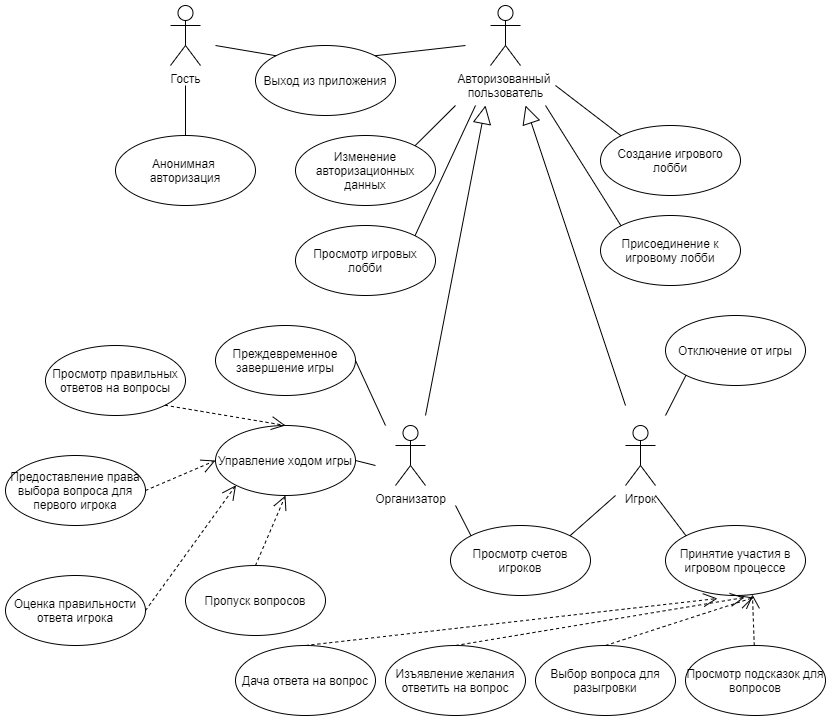
\includegraphics[scale=0.75]{attachments/use_case_model_game.png}
	\caption{Диаграмма вариантов использования игрового клиента}
	\label{fig:domain:model:use_cases:model_game}
\end{figure}

Рассмотрим подробно представленные на рисунке прецеденты.

\emph{Анонимная авторизация} -- функция, которая доступна для роли \linebreak<<Гость>> (пользователь, не авторизованный в системе). 
В качестве данных для авторизации используется псевдоним и аватар, при этом проверок на уникальность не производится, так как в ином случае нарушается анонимность процесса.

Неавторизованный пользователь, как и авторизованный может в любой момент выйти из приложения.

После авторизации пользователь получает доступ к \emph{изменению авторизационных данных}, \emph{просмотру активных игровых лобби}, 
\emph{созданию игрового лобби}, \emph{присоединению к игровому лобби}.
Измение авторизационных данных позволит пользователю изменить свой псевдоним или аватар, если ему не нравится его текущий.
Просмотр активных игровых лобби позволяет всем авторизованным пользователям найти себе лобби для игры по сети. Перед тем, как лобби появится в списке, организатор должен его
создать. После присоединения к лобби пользователь получает роль игрока.
Создание игрового лобби необходимо для того, чтобы другие игроки могли присоединится к викторине. После создания лобби пользователь получает роль организатора. Для создания
лобби необходимо выбрать один из заранее созданных пакетов вопросов.

Основная функциональность системы предусматривается для непосредственных участников игрового процесса: игроков и организатора. 

Одной из самых главных функций, которую использует организатор, является \emph{управление игровым процессом}. Сюда входят такие функции как 
\emph{предоставление права выбора вопроса для первого игрока} и \emph{оценка правильности ответа игрока}. Так как игра имеет пошаговый характер, то необходимо выбрать того,
кто из игроков должен выбрать первый вопрос. Эта одна из задач организатора. В ходе игрового процесса игроки дают ответы на самые разные вопросы, ни один человек 
не может знать ответы на абсолютно все, поэтому на плечи организатора ложится задача по определению правильности ответа игрока. От его решений зависит исход всей викторины. 
В качестве помощи оргизатору приложение отображает \emph{правильный ответ} на текущий вопрос, что облегчает процесс оценки правильности ответов игроков.
Таким образом организатор является ключевой ролью в обеспечении должного уровня качества проведения викторины и уровня эмоций, получаемых в игровом процессе. Вспомогательным
инструментом организатора является возможность \emph{пропустить вопрос} если никто из игроков не знает ответа, в таком случае очки не вычитаются.

Самой главной функцией, которую использует игрок, является участие в игровом процессе. В него входят такие подфункции, как \emph{выбор вопроса для разыгровки},
\emph{изъявление желания дать ответ на вопрос}, \emph{дача ответа на вопрос}, \emph{передача вопроса с секретом другому игроку}, \emph{cоздание ставки в вопросе со ставкой}.
Выбор вопроса для разыгровки прямым образом влияет на сложность самого вопроса: как правило вопросы с большей наградой имеют повышенную сложность. Для того, чтобы дать понять
организатору, что игрок хочет ответить на вопрос, можно воспользоваться функцией изъявляния желания. Если игрок это сделал раньше других, то он получает право ответа на вопрос.
Здесь стоит обратить внимание, что игрок может изъявить желание, но позже не дать ответа из-за волнения или осознания того, что ответа он не знает. В таком случае отказ от ответа 
приравнивается к неправильному ответу с соответствующими вычетами из игрового баланса. Все игроки видят \emph{небольшую подсказку} к ответу на вопрос, которая позволяет убрать некоторые 
сомнения, в случае если составитель викторины не слишком ясно составил вопросы.

Диаграмма вариантов использования программного средства по созданию пакетов вопросов, представлена на рисунке~\ref{fig:domain:model:use_cases:model_test}.

\begin{sidewaysfigure}[!ht]
\centering
	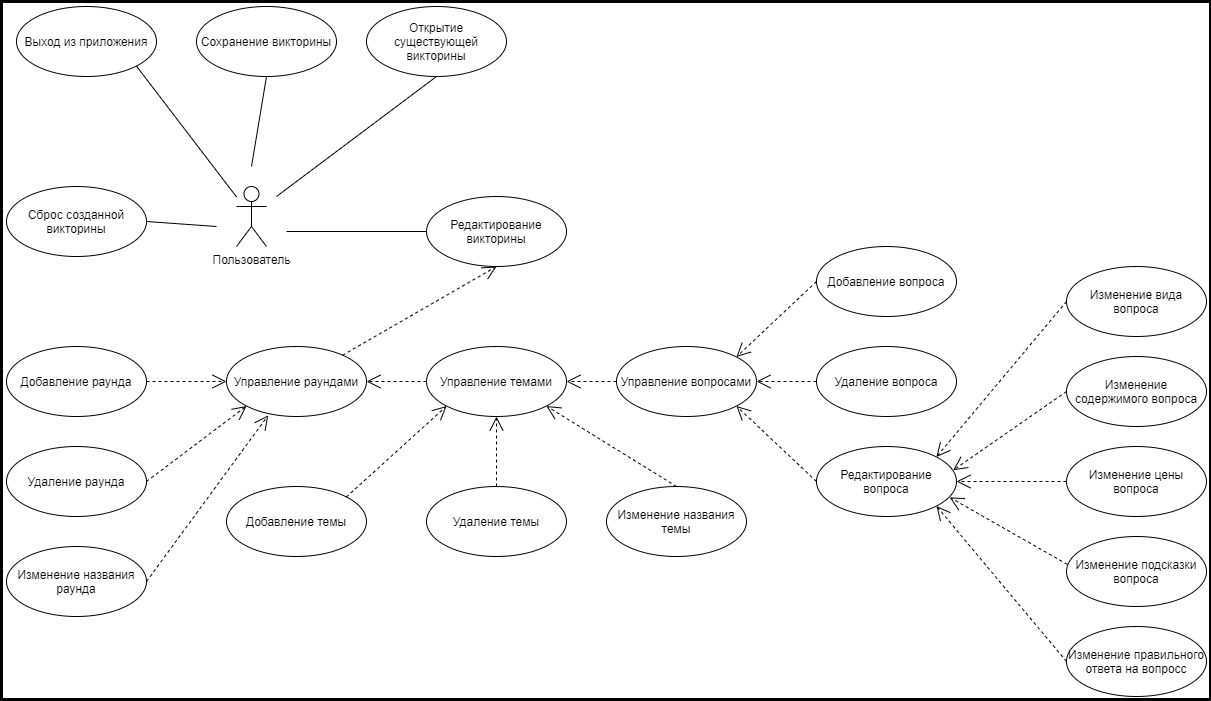
\includegraphics[scale=0.75]{attachments/use_case_model_test.png}
	\caption{Диаграмма вариантов использования ПС создания пакетов с вопросами}
	\label{fig:domain:model:use_cases:model_test}
\end{sidewaysfigure}

\clearpage

Для выполнения поставленной задачи проектируются следующие фун-кции:

\begin{itemize}
	\item \emph{редактирование викторины}, что позволяет создавать комплексный пакет вопросов, содержащий множество раундов и тем;
	\item \emph{сохранение викторины}, что позволяет сохранить результат редактирования на диск с целью дальнейшей доработки или для игры на клиенте;
	\item \emph{открытие существующей викторины}, что означает возможность открыть ранее сохраненный результат редактирования викторины для дальнейших изменений.
\end{itemize}

Создание пакетов вопросов, является неотъемлемой частью работы программного средства: созданные пакеты в дальнейшем интерпретируются клиентом и позволяют участникам принять
участие в игровом опыте. Достоинством такого подхода является возможность делиться викторинами путем передачи файла.

\subsection{Разработка спецификации функциональных требований}
\label{sec:domain:specification}

С учетом требований, определенных в подразделе \ref{sec:analysis:requirements}, необходимо детализировать функциональные требования для проектируемого программного средства.

\subsubsection{} Функция анонимной авторизации
\label{sec:domain:specification:signin}

Функция авторизации должна быть реализована с учетом следующих требований:

\begin{enumerate}
	\item процесс авторизации инициируется пользователем системы (на рисунке~\ref{fig:domain:model:use_cases:model_game} представлен в виде роли <<Гость>>);
	\item функция реализуется собственными средствами без обращения к вне\-ш\-ним поставщикам;
	\item для авторизации пользователь обязан предоставить псевдоним и выбрать аватар;
	\item уникальность псевдонима и аватара не проверяется;
	\item должна быть предусмотрена возможность смены псевдонима и аватара после авторизации.
\end{enumerate}

\subsubsection{} Система ролей
\label{sec:domain:specification:roles}

При реализации системы ролей следует учесть требования:

\begin{enumerate}
	\item должны быть реализованы следующие роли:
	\begin{enumerate}
		\item игрок;
		\item организатор.
	\end{enumerate}
	\item организатор должен иметь возможность управлять игровым процессом;
	\item для получения роли организатора, пользователь должен создать игровое лобби с выбранным пакетом вопросов;
	\item игрок должен иметь возможность непосредственно принимать \linebreak участие в игровом процессе;
	\item для получения роли игрока, авторизованный пользователь должен присоединится к игровому лобби;
	\item должна быть реализована возможность смены роли путем отключения от лобби и создания/присоединения к новому.
\end{enumerate}

\subsubsection{} Функция просмотра списка игровых лобби
\label{sec:domain:specification:view_lobbies}

Просмотр списка игровых лобби входит в число основных функций разрабатываемого приложения. При реализации данной функции необходимо учесть следующие требования:

\begin{enumerate}
	\item необходимо обеспечить отображение списка лобби в виде последовательного списка, отсортированного в порядке убывания дат;
	\item список отображает все лобби, к которым можно подключится, т. е. которые еще активны;
	\item в списке для каждого лобби должна быть отображена следующая информация:
	\begin{enumerate}
		\item название лобби;
		\item псевдоним организатора;
		\item количество игроков в лобби;
		\item максимальное количество игроков;
		\item защита паролем.
	\end{enumerate}
	\item список должен автоматически подгружаться используя API сервиса-координатора. 
\end{enumerate}

\subsubsection{} Функция создания игрового лобби
\label{sec:domain:specification:create_lobby}

Функция создания игрового лобби должна быть реализована с учетом следующих требований:

\begin{enumerate}
	\item для создания лобби необходимо выбрать заранее созданный пакет вопросов;
	\item в настройках можно задать следующие параметры:
	\begin{enumerate}
		\item название лобби;
		\item пароль;
		\item максимальное количество игроков.
	\end{enumerate}
\end{enumerate}

\subsubsection{} Функция управления игровым процессом
\label{sec:domain:specification:control}

Функция управления игровым процессом является ключевой. При ее реализации должны быть учтены следующие требования:

\begin{enumerate}
	\item только организатор может управлять игровым процессом;
	\item при проверке правильности ответа, организатор должен видеть сноску с правильным ответом от составителя вопроса;
	\item в случае правильного ответа игроку начисляются очки;
	\item в случае неправильного ответа игроку снимаются очки;
	\item в случае преждевременного завершения игры победитель не определяется.
\end{enumerate}

\subsubsection{} Функция принятия участия в игровом процессе
\label{sec:domain:specification:play}

Функция принятия участия в игровом процессе также является ключевой. При ее реализации должны быть учтены следующие требования:

\begin{enumerate}
	\item участие может принимать только игрок;
	\item можно выбирать вопрос только в том случае, если у игрока есть право выбора;
	\item игрок имеет право как изъявить желание ответить на вопрос, так и не изъявлять его;
	\item время ответа на вопрос контролируется организатором;
	\item во время ответа на вопрос игроки должны видеть подсказку к ответу;
\end{enumerate}

\subsubsection{} Функция редактирования викторин
\label{sec:domain:specification:edit}

Следующая группа требований относится к деятельности пользователя, создающего набор вопросов:

\begin{enumerate}
	\item каждый вопрос имеет следующий базовый набор данных:
	\begin{enumerate}
		\item содержимое и тип содержимого вопроса;
		\item цена вопроса;
		\item правильный ответ для организатора;
		\item подсказка к ответу для игроков.
	\end{enumerate}
	\item должна быть возможность изменять общее количество раундов в викторине; 
	\item должна быть возможность изменять количество тем в каждом раунде;
	\item должна быть возможность изменять количество вопросов в каждой теме;
	\item должна быть возможность открытия/сохранения викторин.
\end{enumerate}